\documentclass[10pt,fleqn]{article} % Default font size and left-justified equations
\usepackage{import}
\usepackage[%
    pdftitle={Energie et puissance d'un smartphone},
    pdfauthor={Geoffrey Vaquette}]{hyperref}
\subimport{../../../../style/}{preambule}
%\fichetrue
\fichefalse

\proftrue
%\proffalse

\tdtrue
%\tdfalse

\courstrue
%\coursfalse

\subimport{../../../../style/}{new_style}
\subimport{../../../../style/}{macros_SII}
\subimport{../../../../style/}{preambule_trou}

\usepackage{siunitx}
% -------------------------------------
% Déclaration des titres
% -------------------------------------

\def\discipline{Enseignement \\Technologique \\ Transversal}
\def\xxtete{Enseignement Technologique Transversal}

\def\classe{1 STI2D}
\def\xxnumpartie{Séquence 2}
\def\xxpartie{Règlement de classe}

\def\xxnumchapitre{Séance 3}
\def\xxchapitre{\hspace{.12cm} Énergies, Puissances et rendement}

\def\xxposongletx{2}
\def\xxposonglettext{1.45}
\def\xxposonglety{23}
\def\xxonglet{Règles}

\def\xxactivite{~}
\def\xxauteur{\textsl{Geoffrey Vaquette}}

\def\xxcompetences{%
\textsl{%
\textbf{Savoirs et compétences :}
\begin{itemize}[label=\ding{112},font=\color{ocre}]
\item CO2.1	Identifier les flux et la forme de l'énergie, caractériser ses transformations et/ou modulations et estimer l'efficacité globale d'un système.
\end{itemize}
%
}}

\def\xxfigures{
\begin{center}

\includegraphics[height=4cm]{images/smartphone.png} \\
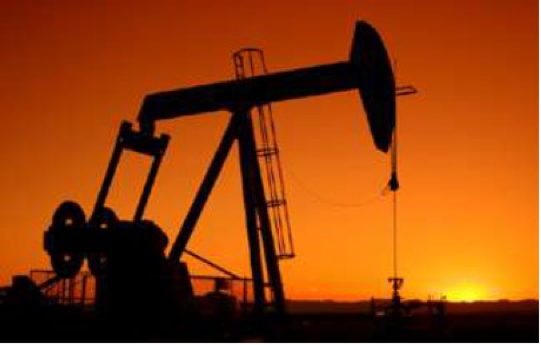
\includegraphics[height=4cm]{images/petrole.png} \\

\includegraphics[height=4cm]{images/gaz.png} \\
\end{center}
}%figues de la page de garde
\def\xxpied{%
Vie de classe \xxactivite%
}

%---------------------------------------------------------------------------

\renewcommand{\RemplirTrou}{true}
\begin{document}
\title{Contrat et règles en classe de STI2D}
\date{Année 2018 - 2019}

Pour l'année 2018-2019, chaque élève, ainsi que le professeur s'engage à respecter les règles suivantes : 
\section{Respect}
\subsection{Droits}
\begin{itemize}
    \item Chaque élève a le droit au respect des autres élèves ainsi que du professeur. 
    \item Le professeur a le droit au respect de chacun des élèves.
\end{itemize}

\subsection{Devoirs}
\begin{itemize}
    \item Chaque individu de la classe s'adresse la parole correctement, poliment, sans vulgarité ni agressivité à l'égard de quiconque. 
    \item Lorsqu'un élève s'adresse au professeur et/ou au reste de la classe, tout le monde l'écoute sans l'interrompre. 
    \item Lorsque le professeur s'adresse aux élèves (pour expliquer un cours, corriger un exercice par exemple), tous les élèves l'écoute.
\end{itemize}

\section{Travail en classe}
\subsection{Droits}
\begin{itemize}
    \item Tout élève a le droit d'écouter et de participer aux cours, aux TDs, aux TPs.
    \item Tout élève a le droit de poser une question pour demander une clarification d'une notion de cours ou d'une question qu'il n'aurait pas comprise. 
    \item Le professeur a le droit d'interroger un élève pour vérifier qu'une notion a bien été comprise.
    \item Le professeur a le droit d'être écouté lorsqu'il s'adresse à la classe. 
    \item Les élèves ont le droit de connaître les modalités d'évaluation ainsi que les résultats des évaluations. 
\end{itemize}
\subsection{Devoirs}
\begin{itemize}
    \item Pour garantir une répartition de la parole, les élèves lèvent la main s'ils veulent la parole. C'est l'enseignant qui distribue  la parole. 
    \item Pour que tout le monde puisse écouter ce qui est dit et travaille dans le calme, un élève qui n'a pas la parole n'est pas autorisé à parler, ni bavarder avec un camarade de classe. 
    \item Le professeur doit répartir la parole de façon équitable, tout en garantissant la bonne avancée du cours. 
    \item Afin de pouvoir suivre le cours, les élèves ont le devoir de prendre des notes et de recopier le cours, les exercices et les corrigés donnés par le professeur. 
    \item L'utilisation du téléphone portable n'est, a-priori, pas autorisée. Si l'élève doit, pour une raison urgente, l'utiliser il doit en demander l'autorisation préalable au professeur.  
    \item Le professeur s'engage à tout faire pour corriger les devoirs rendus avant la séance suivante et s'engage à le rendre au plus tard sous 15 jours. 
\end{itemize}

\section{Assiduité}
\subsection{Droits}
\begin{itemize}
    \item Les élèves et le professeur ont le droit de sortir à la dernière sonnerie de la séance de cours.
    \item Les élèves et le professeurs ont le droit de commencer le cours à l'heure, sans perturbation extérieure. 
\end{itemize}

\subsection{Devoirs}
\begin{itemize}
    \item Afin de débuter le cours le plus rapidement possible, les élèves doivent entrer dans le calme, s'asseoir à leur place et sortir leurs affaires de cours dès que le professeur les invite à entrer en classe. 
    \item Pour ne pas perturber le cours, les élèves ne sont plus autorisés à entrer en classe (sans justification écrite et valable) une fois que l'appel a été fait. 
    \item En cas d'absence, l'élève doit rattraper le cours sur pronote ou auprès d'un autre élève AVANT la séance suivante. 
    \item Le professeur doit mettre sur pronote les documents distribués et utilisés en classe, afin que les élèves puissent y avoir accès. 
\end{itemize}

\section{Matériel}
\subsection{Droits}
\begin{itemize}
    \item Tout élève a le droit d'avoir les supports de cours, TD et TP de la séance. 
    \item Toute personne a le droit au respect de ses affaires tant qu'il n'en fait pas un usage non autorisé.
    \item L'élève a le choix de l'organisation de ses documents, tant qu'ils sont facilement et rapidement accessibles à tout moment. 
    \item Le professeur peut exiger qu'un ou plusieurs élèves apportent leur classeur (ou cahier ou porte-vues) contenant tous les documents de l'année, pour vérifier son organisation et la présence de tous les documents. 
    \item S'il considère que la façon de trier et d'organiser les documents d'un élève n'est pas satisfaisante, le professeur est en droit d'exiger une autre organisation. 
\end{itemize}
\subsection{Devoirs}
\begin{itemize}
    \item Tout élève doit avoir avec lui de quoi écrire (feuille et stylo) ainsi que l'ensemble des documents de la séquence en cours. 
    \item Les élèves doivent conserver, de manière organisée et facilement accessible, la totalité des documents utilisés en cours, jusqu'à la fin de l'année scolaire (et idéalement jusqu'au baccalauréat). 
    \item Pour prévenir toute perte de document, l'utilisation d'une pochette pour conserver les documents, n'est pas autorisée. 
    
\end{itemize}

\section{Punition et sanctions}
Tout manquement par un élève à l'un des devoirs cités dans ce document ou dans le règlement intérieur du lycée l'expose à une punition ou une sanction. 

Ces punitions ou sanctions peuvent prendre la forme d'une observation dans le carnet de correspondance à faire signer par le référent légal de l'élève, d'heures de retenues avec travail supplémentaire, d'exclusion de cours et/ou de privation d'un droit cité dans ce document. 

\subsection{Punitions et sanctions types}
\begin{itemize}
    \item  Les bavardages, les amusements en cours seront sanctionnés après un premier avertissement oral. 
    \item L'utilisation excessive du téléphone portable sera sanctionnée et celui-ci confisqué après un premier avertissement oral. 
    \item Sur chaque trimestre, la première fois qu'un appareil sera confisqué, il sera rendu à la fin de la séance. A partir de la deuxième fois, il sera remis au CPE ou au proviseur. 
    \item L'absence du matériel nécessaire à la prise de note ou l'absence d'un travail donné à la maison sera sanctionnée la première fois par une observation dans le carnet de correspondance. La deuxième fois, l'élève pourra être exclu du cours et/ou se voir attribuer une heure de retenue avec travail supplémentaire. 
\end{itemize}

\section{Autre}
\end{document}
